%!TEX root=../../main.tex
\section{Datenschnittstelle und Webseitenlogik}
Die Schnittstelle zwischen Frontend und Backend wird mittels JavaScript-Framework umgesetzt. Wie in Kapitel \hyperref[sec:rfoster_fazit]{5.3.5} beschrieben, wird hierfür VueJS verwendet. VueJS bietet viele passende Funktionen und Features, um  eine solche Webseite umzusetzen.
\subsection{Webseitenlogik}
\label{sec:webseitenlogik}
Die Webseite wird mittels Vue-Komponenten aufgebaut werden. Eine Seite besteht aus einer Hauptkomponente und möglicherweise noch zusätzlichen Nebenkomponenten. Die Struktur der einzelnen Komponenten und Links der Webseite soll wie folgt aussehen:
\begin{figure}[H]
	\centering
	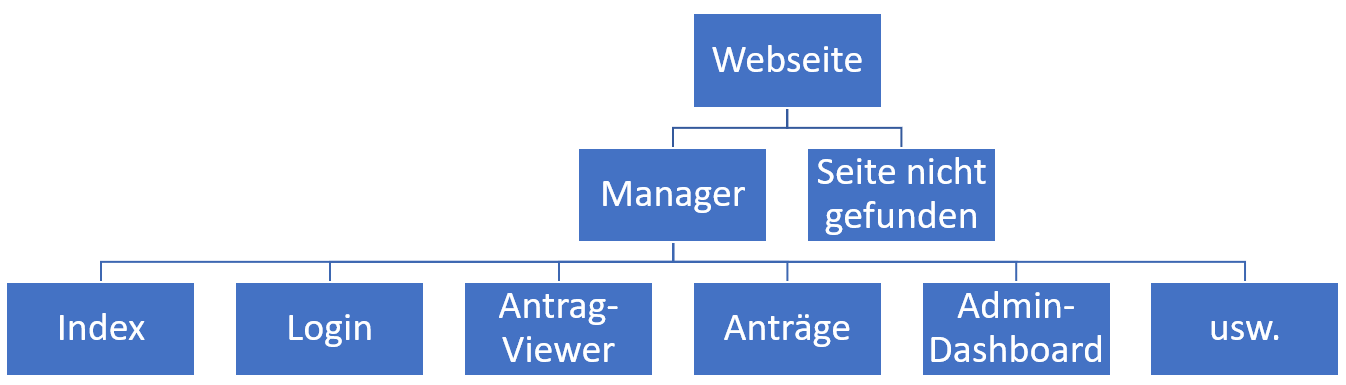
\includegraphics[width=0.8\linewidth]{images/Webseite_hierarchie}
	\caption[Hierarchie der Webseite]{Übersicht der Hierarchie der Webseite}
	\label{fig:webseitehierachie}
\end{figure}

\subsubsection{Seite nicht gefunden}
\label{sec:not_found}
Wird ein Link eingegeben, welcher nicht auf die Seite selbst oder eine definierte Unterseite verweist, wird eine Seite geladen, bei der der Benutzer darauf hingewiesen wird, dass kein korrekten Link eingegeben wurde.
\begin{figure}[H]
	\centering
	
\includegraphics[width=0.6\linewidth]{images/page_not_found}
	\caption[Seite nicht gefunden]{Seite nicht gefunden}
	\label{fig:pagenotfound}
\end{figure}

\subsubsection{Manager}
Der \textit{Manager} ist der Hauptbestandteil der Webseite. Er beinhaltet alle einzelnen Seiten und zeigt immer die gewünschte Seite an. In dem \textit{Manager} werden auch Cookie-Einstellungen und Rechte gespeichert. Fast alle Komponenten werden dem Manager untergeordnet. Der \textit{Manager} ist auch dafür verantwortlich, Daten zwischen Komponenten zu übermitteln.

\subsubsection{Komponenten}
Einzelne Komponenten laden die Daten eigenständig aus dem Backend. Dies ist eine Maßnahme, um den \textit{Manager} nicht mit Funktionen zu überladen und damit nicht bei jedem Aufruf Daten vom \textit{Manager} an die einzelnen Komponenten gesendet werden müssen.\\
Im dem Fall, dass eine Komponente Daten an eine weitere Komponente sendet, wird diese Kommunikation vom \textit{Manager} übernommen.

\subsubsection{Antrag-Viewer}
Es soll eine weitere Seite vorhanden sein, auf die man durch einen Link gelangen kann. Auf dieser Seite soll es möglich sein, einen Antrag per ID anzeigen zu lassen. Da dieser separate Link technisch auf der selben Ebene wie der \textit{Manager} ist, wird dafür gesorgt, dass dieser Link dem \textit{Manager} nahtlos untergeordnet ist. Der \textit{Antrag-Viewer} ist nur verwendbar, sofern der Benutzer angemeldet ist und auch die Berechtigung hat, diesen Antrag zu betrachten.
\\\\
Wird in den Parametern des Links bereits spezifiziert, welcher Antrag geöffnet werden soll, wird dem Benutzer nach der Anmeldung dieser Antrag angezeigt. Es können nur jene Anträge angezeigt werden, zu denen der Benutzer die erforderlichen Berechtigungen besitzt. Besitzt der Benutzer nicht die erforderlichen Berechtigungen, wird eine Fehlermeldung ausgegeben.

\subsubsection{Navigation}
Da fast alle Komponenten dem Manager untergeordnet sind, ist es auch die Verantwortung des Managers die Navigation zu steuern. Dazu gibt es eine zentrale Funktion im Manager, welche die derzeit geladene Seite verändern kann. Des Weiteren werden die benötigten Informationen geladen bzw. erstellt, welche die Komponenten benötigen.
\\\\
Die Funktion zum Verändern der derzeitigen Anzeige wird von den untergeordneten Komponenten aufgerufen. Hinzu kommt, dass mit dem Aufruf der Funktion auch spezifiziert wird, welche Seite geladen werden soll. Spezielle Seiten, wie z.B: der \textit{Antrag-Viewer}, benötigen zusätzlichen Informationen, welche über diese Funktion mitgegeben werden.

\subsubsection{Features}
\label{sec:feature}
Es sollen auch Funktionen implementiert werden, welche das Benützen der Webseite erleichtern.
\\\\
Es soll möglich sein, bei erneutem Laden der Webseite auf die zuletzt geöffnete Seite zu gelangen. Beim Beenden des Browsers speichert die Webseite die aktuelle Seite und lädt diese bei erneutem Aufrufen der Webseite automatisch.
\\\\
Es ist durch die Browser-Pfeile auch möglich zwischen den Seiten zu navigieren. Dies ist wichtig, da durch versehentliches wechseln der Komponente ein Benutzer möglichst schnell wieder auf die vorherige Seite gelangen soll. Durch die Implementierung der Browser-Pfeile ist es möglich intuitiv auf die vorherige Seite zu wechseln. Andere Funktionen, welche die selbe Funktionalität haben, werden durch diese Implementierung auch unterstützt.
\newpage
\subsection{Daten laden}
Auf den Seiten, wo es benötigt wird, werden über Funktionen des Frameworks dynamisch Komponenten erstellt und geladen. Der Prozess Daten aus dem Backend zu laden wird in folgender Grafik beschrieben:
\begin{figure}[H]
	\centering
	
\includegraphics[width=0.8\linewidth]{images/Prozess_Daten_laden}
	\caption[Prozess der Daten zur Anzeige]{Übersicht über den Prozess, welcher Daten aus dem Backend lädt}
	\label{fig:prozessdatenladen}
\end{figure}

\subsubsection{Webseite aufrufen}
Die Webseite wird aufgerufen und der Benutzer bekommt die Startseite angezeigt.

\subsubsection{Datenabfrage erstellen und Daten erhalten}
Auf der Startseite der Webseite werden die neuesten Nachrichten angezeigt, welche für den Lehrer relevant sind. Hierfür müssen aus dem Backend Daten geladen werden. Dies erfolgt über eine Abfrage, welche aus dem Frontend gesendet wird, Daten ausliest und diese dann verwendet, um Komponenten zu erstellen.

\subsubsection{Komponenten erstellen}
Die geladenen Daten aus dem Backend werden mittels Einbindung der Variablen in einzelne Komponenten eingebunden.\\
Seiten, auf denen viele gleiche Komponenten sind, werden mittels Schleifen erstellt. Diese sorgen dafür, dass nicht zu viele Komponenten auf der Seite geladen sind, wenn diese nicht gebraucht werden.
Ein Beispiel hierfür sind die neuen Nachrichten, welche in folgender Grafik gezeigt werden:
\begin{figure}[H]
	\centering
	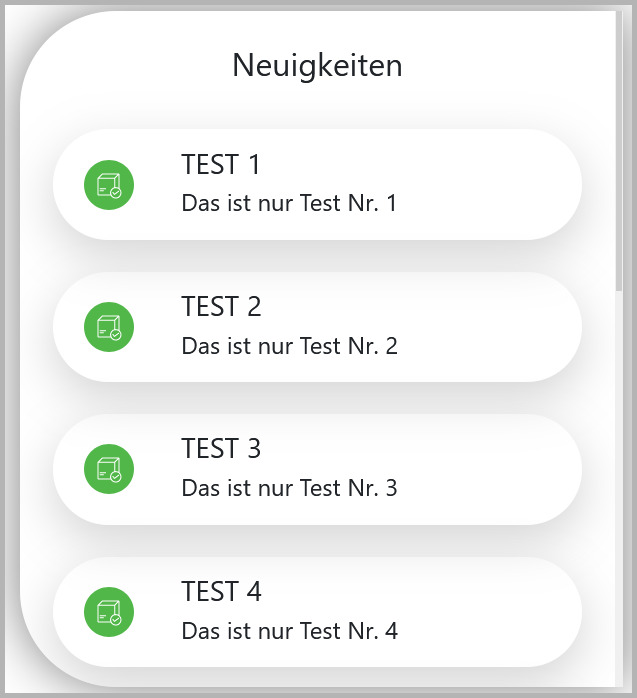
\includegraphics[width=0.3\linewidth]{images/messages_index}
	\caption[Neue Nachrichten]{Grafik der neuen Nachrichten}
	\label{fig:messagesindex}
\end{figure}

\subsubsection{Komponenten anzeigen}
Die bereits erstellten Komponenten werden über die Einbindung in der Webseite angezeigt. Dies kann durch einfache Implementierung bei einzelnen Komponenten erreicht werden.\\
Durch die Schleife können auch die Komponenten angezeigt werden. Diese ordnet alle Komponenten hintereinander  und zeigt diese an.\\
Bei den Nachrichten kann man sich jede Nachricht als eigene Komponente vorstellen, welche jeweils erstellt und danach angezeigt wird.
%\newpage
\subsection{Befehle senden}
Die Webseite besitzt auch einige Aktionen, die von Benutzern ausgeführt werden können. Diese müssen je nach Aktion eine neue Seite aufrufen oder einen Befehl an das Backend senden.

\begin{figure}[H]
	\centering
	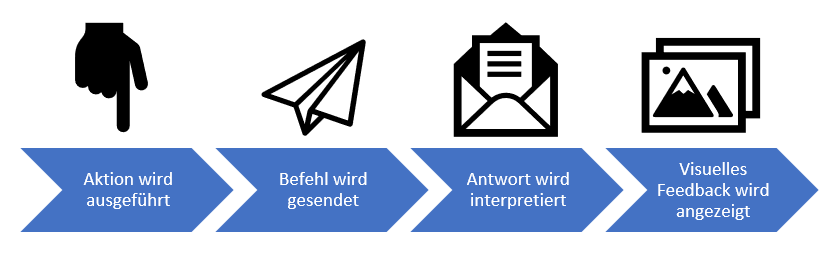
\includegraphics[width=0.8\linewidth]{images/Prozess_Befehl_senden}
	\caption[Prozess der Befehlssendung]{Übersicht über den Prozess, welcher Befehle an das Backend sendet}
	\label{fig:prozessbefehlsenden}
\end{figure}

\subsubsection{Aktion ausführen}
Eine Aktion wird ausgeführt, wenn z.B. auf eine Komponente gedrückt wird. Dies ruft eine Funktion auf, bei der eine Anfrage erstellt wird.

\subsubsection{Befehl senden}
Eine Anfrage beinhaltet alle wichtigen Informationen des Befehls für das Backend. Sie wird anschließend an das Backend gesendet, um dort abgearbeitet zu werden.

\subsubsection{Antwort interpretieren}
Sobald das Backend den Befehl in der Anfrage ausgeführt hat, wird eine Antwort an das Frontend gesendet und soll dort interpretiert werden. Die Interpretation der Antwort soll durch den Status der Antwort geschehen. Der Status der Antwort ist ein Code, welcher aussagt, ob der Befehl funktioniert hat oder fehlgeschlagen ist. Sollte der Befehl fehlschlagen, so deutet der Code auf den genauen Fehlergrund hin.

\subsubsection{Information anzeigen}
Tritt ein Fehler auf, soll dies dem Benutzer offensichtlich mitgeteilt werden. Sollte kein Fehler auftreten, soll das dem Benutzer je nach Befehl auf unterschiedliche Weise mitgeteilt werden.\\
Um weiterhin das Beispiel zu nutzen: Wenn eine Nachricht gelöscht wird, wird dem Benutzer mitgeteilt, dass die Nachricht gelöscht worden ist, indem diese verschwindet.